\section{MPI}\label{sec:mpi}
\subsection{Implementation}
Implementing this algorithm in MPI requires decomposing the problem into sub
parts, similar to the idea of domain decomposition from the last project. We
drew inspiration from previous work with distance-vector routing using
Bellman$-$Ford in determining shortest distances between routers. In that
algorithm, each router sends its distances to all other routers (each time
there is a change) to its neighbors which then use that information to update
their own distances. This continues until no routers have changed distances.

In our case we do not necessarily have a single thread per node, as there maybe
not be enough available hardware threads. Instead each ''router'' is an MPI
rank and is responsible for a set of nodes rather than a single node. Each MPI
rank calculates the minimum distance to each of its nodes from all other nodes
going through some node between 1 and $N$. Each rank also determines if any
distances have changed. All MPI ranks then synchronize, to gather distances
from one another and determine if any distances have changed (if none stop then
we are done and the ''master'' rank (rank 0) outputs checksum and timing
information). To determine if any distances have changed we use
\texttt{mpi\_allreduce} on each rank's done variable. To synchronize distances
across all ranks we use \texttt{mpi\_allgather} which sends each rank's
distances to all other ranks and collects them from every rank, including
itself, into a single buffer. Our implementation is in \texttt{path-mpi.c}.

\subsection{Performance}
\begin{figure}[h]
  \centering
  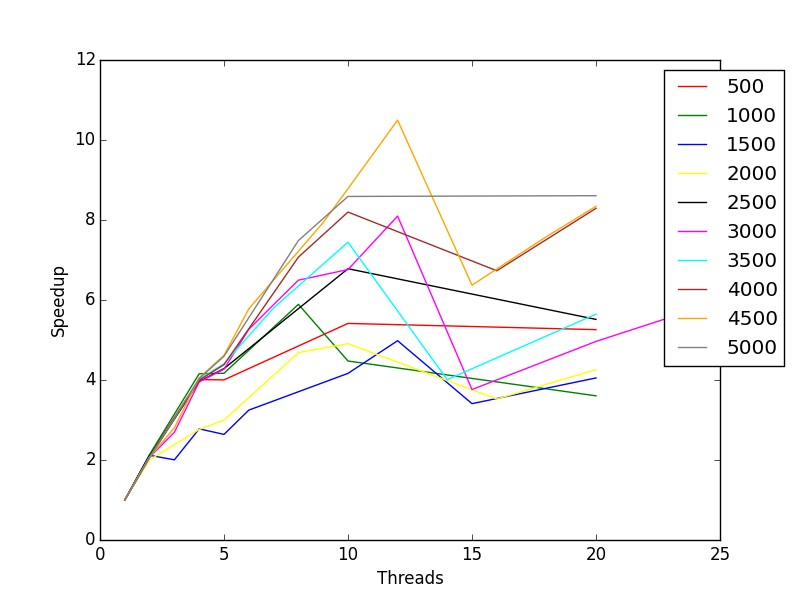
\includegraphics[width=0.68\textwidth] {plots/1}
  \caption{%
    Strong scaling speedup of our MPI code as number of threads (ranks)
    increase. Baseline for calculating speedup is MPI with 1 rank
  }
  \label{aload0}
\end{figure}

\begin{figure}[h]
  \centering
  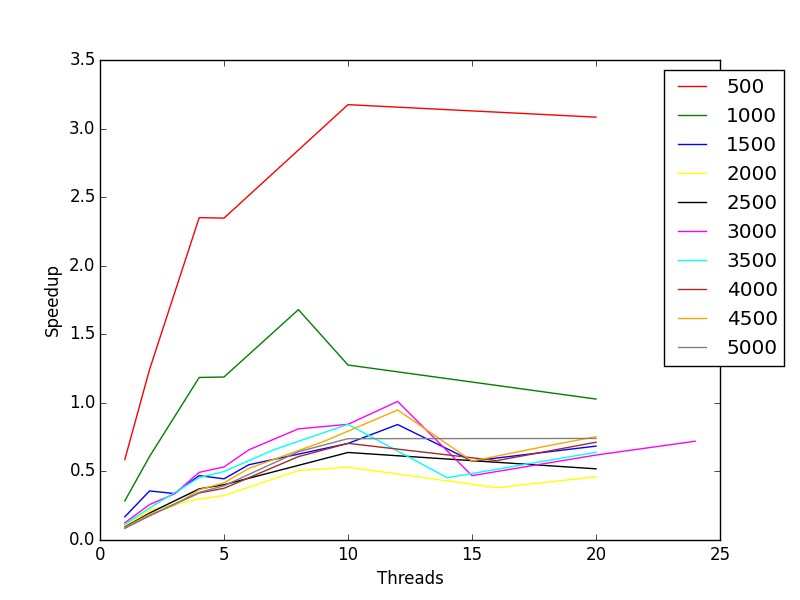
\includegraphics[width=0.68\textwidth] {plots/2}
  \caption{%
    Strong scaling speedup of our MPI code as number of threads (ranks)
    increase. Baseline for calculating speedup is OMP with 24 threads.
  }
  \label{aload1}
\end{figure}

In Figure 1 we show the results of running our MPI code for various problem
sizes and showing how speedup scales as we increase the number of MPI ranks.
Larger problems tend to have greater speedup than smaller ones. This makes
sense as when we increase problem size less time increase spent in
synchronization as compared to actually computation. This means as we increase
the number of ranks we should continue to speedup as synchronization does not
grow as quickly. The drop seen in speedup when we go beyond 12 ranks is due to
now having ranks on 2 chips rather than 1 chip. This increases communication
overhead during synchronization which results in a lower overall speedup
despite having more cores.

We also compared the performance of our MPI code with that of OMP, where omp
was allowed to use all 24 threads (Figure 2) in a strong scaling study. We see
that for the two smallest problem sizes our code outperforms OMP as ranks
increase beyond 1, but for larger problems our MPI code always performs worse.
This is unsurprising as for small problems OMP will have a lot of
synchronization overhead for 24 threads while MPI will do better with a smaller
problem. However, when the problem is larger MPI, which has a larger
synchronization overhead than OMP, MPI performs worse.
